%------------------------------------------------------------------------------
% solution.tex
%
% This illustrates the solution proposed. 
%------------------------------------------------------------------------------
\chapter*{soluzione proposta}
\addcontentsline{toc}{chapter}{Soluzione proposta}
\label{soluzione-proposta}
In questo capitolo sono fornite informazioni in merito alla soluzione proposta dallo studente.

\section*{tecnologie}
\addcontentsline{toc}{section}{Tecnologie}
\label{soluzione-proposta-tecnologie}
Per l'implementazione della soluzione proposta si sono utilizzate le seguenti tecnologie:

\begin{itemize}
\item{il linguaggio Scala con l'utilizzo delle librerie dell'Akka \english{framework} per l'implementazione del modulo ``\english{core}'' del sistema;}
\item{il linguaggio Scala con l'utilizzo del \english{Play framework} per l'implementazione del modulo ``monitor'' del sistema.}
\end{itemize}

\begin{figure}[h!]
\begin{subfigure}{0.5\textwidth}
\centering

\includegraphics[width=0.6\linewidth]{images/solution/scala.png}
\caption{Linguaggio Scala}
\end{subfigure}
\begin{subfigure}{0.5\textwidth}
\centering

\includegraphics[width=0.3\linewidth]{images/solution/akka.png}
\caption{Akka framework}
\end{subfigure}
\\
\begin{subfigure}{0.5\textwidth}
\centering

\includegraphics[width=0.3\linewidth]{images/solution/play.png}
\caption{Play framework}
\end{subfigure}
\begin{subfigure}{0.5\textwidth}
\centering

\includegraphics[width=0.4\linewidth]{images/solution/websocket.png}
\caption{web socket}
\end{subfigure}
\caption{Tecnologie utilizzate per il simulatore}
\label{soluzione-proposta-tecnologie-tecnologie-usate}
\end{figure}

L'utilizzo del linguaggio Scala si è preferito cosi da poter eseguire il simulatore su architetture differenti in quanto, l'eseguibile prodotto è formato da codice \english{bytecode} eseguibile sulle \ac{jvm}. Nonostante si basi sulla \ac{jvm} come \english{runtime} di esecuzione, si sono sfruttate le librerie del \english{framework} akka per l'utilizzo del modello ad attori per la gestione della concorrenza, un modello più valido rispetto alla gestione della concorrenza fornita dal linguaggio Java.

Come precedentemente affermato, data la proprietà di \english{location transparency} fornita dal modello ad attori non è stato necessario corredare il modulo \english{core} di un \english{middleware} esterno per la gestione delle comunicazioni tra i diversi nodi che lo compongono.

Infine si è scelto di utilizzare il \english{Play framework} per la costruzione di una \english{web application} che sia in grado di visualizzare lo stato corrente della simulazione. L'utilizzo di questa tecnologia e stato scelto poiché rende possibile il collegamento con il modulo \english{core} attraverso l'utilizzo di \english{web socket}. L'utilizzo di queste ultime consente la creazione di un canale \english{full-duplex} tra \english{client} e \english{server} che consente al  \english{core} di poter inviare eventi rilevanti alla grafica senza che quest'ultima esegua azioni di \english{polling} per rimanere aggiornata.

Lo svincolo dalla tecnica del \english{polling} consente di avere un sistema che sia in grado di reggere un numero molto superiore di \english{client} che necessitano di visualizzare lo stato della simulazione.

\section*{architettura del sistema}
\addcontentsline{toc}{section}{Architettura del sistema}
\label{soluzione-proposta-architettura}
In Figura \ref{soluzione-proposta-architettura-immagine} è visualizzato un diagramma di alto livello\footnote{Si vuole far notare al lettore che nel diagramma sono presenti, per semplicità, solo le connessioni più importanti} illustrante l'architettura del sistema costruito. Viene ora fornita una breve spiegazione degli attori principali che prendono parte al sistema.

\begin{figure}[h!]
\centering
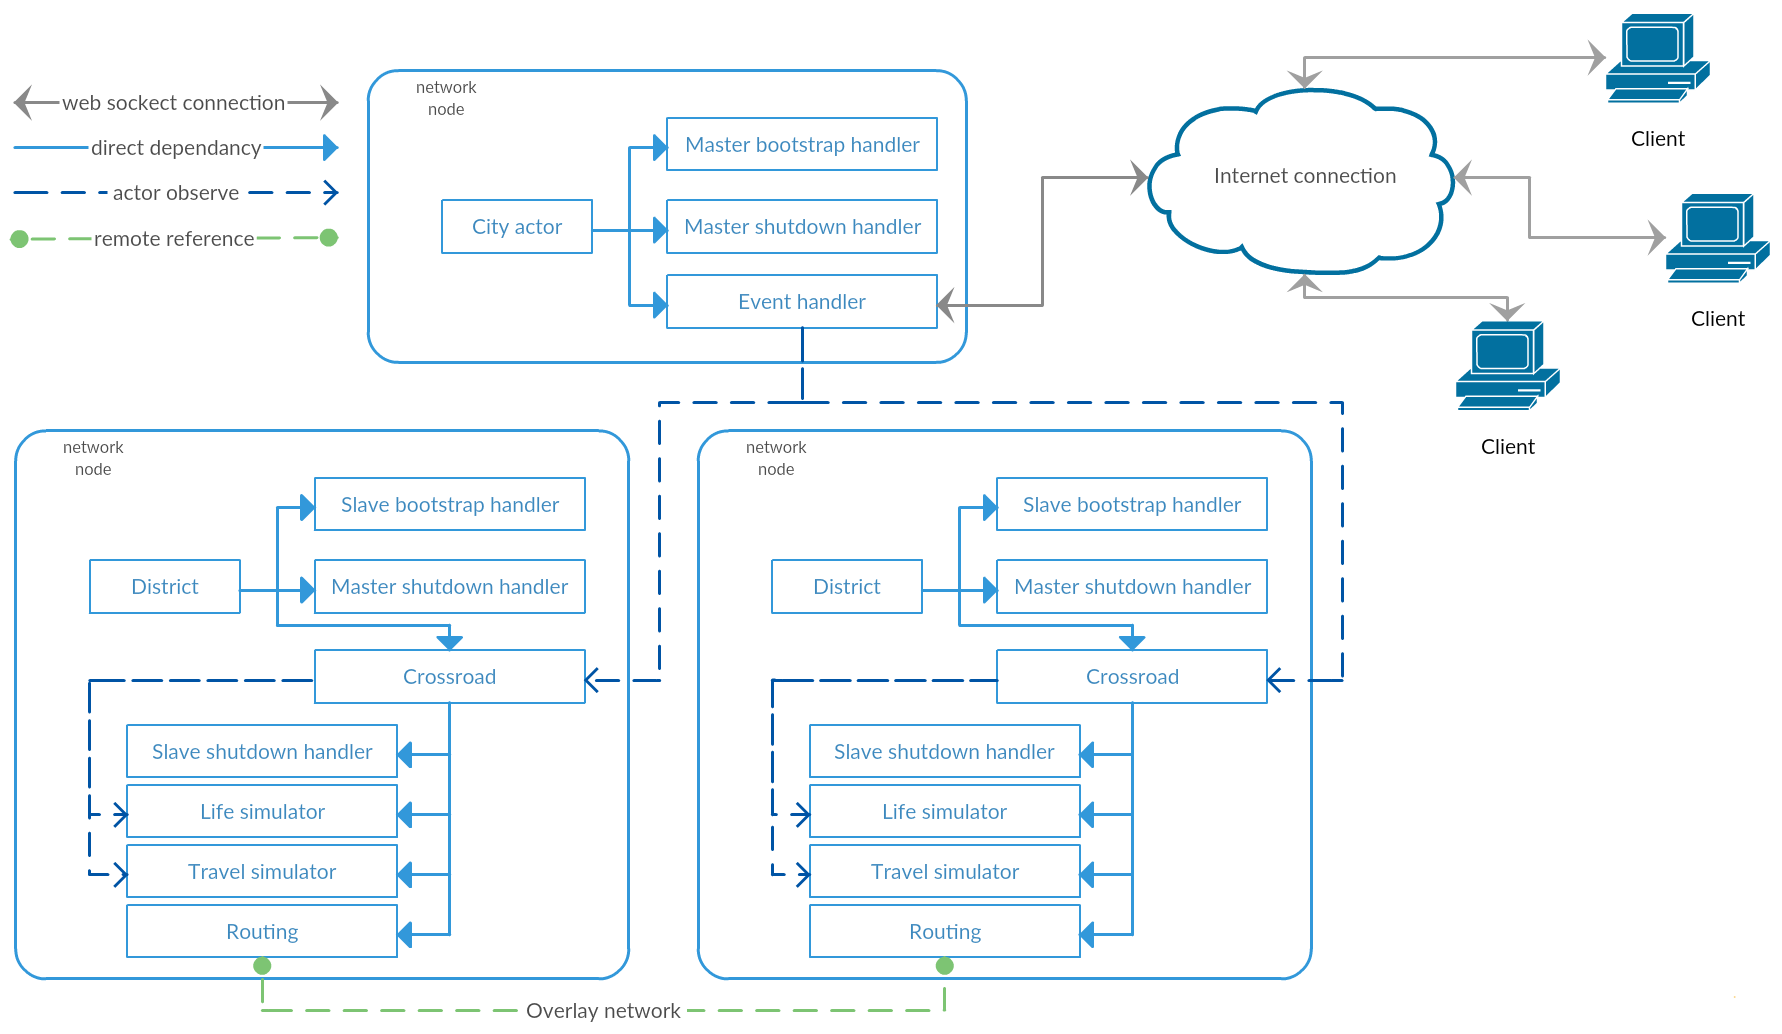
\includegraphics[scale=0.25]{images/solution/architecture.png}
\caption{Architettura del sistema}
\label{soluzione-proposta-architettura-immagine}
\end{figure}

\subsection*{attore ``city''}
\addcontentsline{toc}{subsection}{Attore ``city''}
\label{soluzione-propoposta-architettura-city}
L'attore amministra l'accesso alla struttura cittadina da parte dei \english{client} ed altre componenti che hanno necessità di dialogare con essa. E' composto dei seguenti attori, ai quali delega compiti specifici:

\begin{itemize}
\item{\english{MasterBootstrapHandler}: il quale gestisce le fasi del protocollo di \english{bootstrap} per l'intera struttura dati;}
\item{\english{MasterShutdownHandler}: il quale gestisce le fasi del protocollo di \english{shutdown} per l'intera struttura dati;}
\item{\english{EventHandler}: il quale riceve ed elabora gli eventi, provenienti dagli incroci, prima di inviarli ai \english{client}.}
\end{itemize}

\subsection*{attore ``master-bootstrap-handler''}
\addcontentsline{toc}{subsection}{Attore ``master-bootstrap-handler''}
\label{soluzione-poposta-architettura-master-bootstrap-handler}
L'attore amministra il \english{bootstrap} dei nodi che gestiranno i quartieri (o distretti) di cui è composta la città. Nel momento in cui esso rileva che l'\english{overlay network} è correttamente settata e che l'attore amministrante lo \english{shutdown} del sistema ha i riferimenti agli attori, esso termina le proprie mansioni cedendo il controllo all'attore ``Città'' per iniziare la fase di popolamento.

\subsection*{attore ``slave-bootstrap-handler''}
\addcontentsline{toc}{subsection}{Attore ``slave-bootstrap-handler''}
\label{soluzione-poposta-architettura-slave-bootstrap-handler}
L'attore amministra il \english{bootstrap} degli incroci che sotto la giurisdizione di un particolare distretto. Nel momento in cui esso rileva che la porzione di \english{overlay network}, gestita dal nodo stesso, è correttamente settata l'attore cessa le proprie mansioni comunicando all'attore ``distretto'' di rimanere in attesa dell'avvio della simulazione.

\subsection*{attore ``master-shutdown-handler''}
\addcontentsline{toc}{subsection}{Attore ``master-shutdown-handler''}
\label{soluzione-proposta-architettura-master-shutdown-handler}
L'attore amministra lo \english{shutdown} sia del nodo contenente l'attore ``città'' che il il nodo contenente l'attore ``distretto''. In particolare quando esso rileva che tutte gli attori di livello inferiore nella gerarchia, gli incroci nel caso degli attori ``distretti'' ed i distretti nel caso dell'attore ``città'', termina il sistema che gestisce e supervisiona gli attori. Come risultato finale si otterrà una chiusura sicura e pulita dell'intero sistema.

Nel caso di future espansioni del simulatore in questo punto è possibile inserire l'algoritmo di salvataggio dello stato del sistema, il quale verrà eseguito a simulazione interrotta e subito prima che il sistema cessi. Il salvataggio dello stato può avvenire implementando l'algoritmo dello \english{snapshot} distribuito determinato da Chandy e Lamport.

\subsection*{attore ``slave-shutdown-handler''}
\addcontentsline{toc}{subsection}{Attore ``slave-shutdown-handler''}
\label{soluzione-proposta-architettura-slave-shutdown-handler}
L'attore amministra lo \english{shutdown} di un singolo incrocio del sistema. Affinché tale attore possa terminare correttamente le proprie mansioni è necessario che gli attori a cui esso delega parte del lavoro di simulazione abbiano terminato le proprie mansioni.

\subsection*{attore ``event-handler''}
\addcontentsline{toc}{subsection}{Attore ``event-handler''}
\label{soluzione-proposta-architettura-event-handler}
L'attore ha il compito di registrarsi come ascoltatore di eventi presso gli incroci che costituiscono la città e di processarli, secondo esigenze specifiche, prima che essi siano inviati alla componente monitor. La traduzione degli eventi dallo stato ``grezzo'' allo stato ``lavorato'' viene delegata ad attori specifici per ogni tipologia di elaborazione a lui dipendenti che forniranno il risultato finale che verrà fornito alla componente monitor.

In Figura \ref{soluzione-proposta-architettura-event-handler-gerarchia} è visibile la gerarchia di attori eventi in carico la costruzione dei pacchetti dati da inviare alla componente ``monitor''. Gestendo, lato servente, tale tipo di computazione si ha la possibilità di costruire clienti più snelli e leggeri, potendo cosi supportare anche quelli con risorse limitate.

\begin{figure}[h!]
\centering
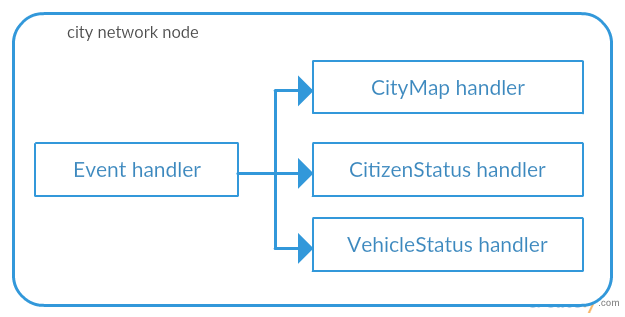
\includegraphics[scale=0.5]{images/solution/event-handler.png}
\caption{Attori aventi il compito della gestione degli eventi per la componente monitor}
\label{soluzione-proposta-architettura-event-handler-gerarchia}
\end{figure}

L'attore ``\english{CityMap handler}'' ha il compito di costruire un pacchetto dati contenente le informazioni che il \english{client} utilizza per visualizzare la mappa della struttura cittadina. Esso fornisce una struttura dati JSON contenente la gerarchia della componenti costituenti la città, ognuna di essa corredata con le coordinate geografiche che il \english{client} utilizzerà per visualizzare la mappa.

L'attore ``\english{CitizenStatus handler}'' ha il compito di costruire delle stringhe testuali che illustrino lo stato attuale di un cittadino nel sistema. Quest'ultimo può trovarsi in:

\begin{itemize}
\item{riposo (sta dormendo presso la propria abitazione);}
\item{alla fermata dell'autobus (se è previsto che esso debba viaggiare tramite un autobus);}
\item{in viaggio;}
\item{lavorando (sta eseguendo le proprie mansioni nel luogo di lavoro).}
\end{itemize}

L'attore ``\english{VehicleStatus handler}'' ha il compito di tradurre lo stato di avanzamento di un veicolo in coordinate geografiche valide relative alla mappa della città in questione.

\subsection*{attore ``district''}
\addcontentsline{toc}{subsection}{Attore ``district''}
\label{soluzione-proposta-architettura-district}
L'attore amministra l'accesso alle componenti che compongono il distretto da parte dell'attore ``city''.

\subsection*{attore ``crossroad''}
\addcontentsline{toc}{subsection}{Attore ``crossroad''}
\label{soluzione-proposta-architettura-crossroad}
L'attore è il vero artefice della simulazione in quanto consente ai veicoli di poter transitare nella città. Le azioni inerenti la simulazione vera e propria sono gestite da attori specifici a lui dipendenti, tra cui si può trovare:

\begin{itemize}
\item{\english{life simulator};}
\item{\english{travel simulator};}
\item{\english{routing}.}
\end{itemize}

Nelle sezioni successive viene fornita una breve descrizione del ruolo assunto da tali attori. Lo stato interno di tale attore contiene invece:

\begin{itemize}
\item{un \keyword{parcheggio} contenente i veicoli in attesa del segnale di avvio simulazione o di avere informazioni di \english{routing} per raggiungere una destinazione;}
\item{una \keyword{fermata dell'autobus}, la quale ospita le persone che attendono il passeggio dell'autobus o che, appena scese dal medesimo, si stanno per recare a compiere le proprie mansioni;}
\item{un \keyword{garage}, il quale contiene le automobili parcheggiate dai rispettivi proprietari mentre questi ultimi stanno compiendo le proprie mansioni.}
\end{itemize}

\subsection*{attore ``life simulator''}
\addcontentsline{toc}{subsection}{Attore ``life simulator''}
\label{soluzione-proposta-architettura-life-simulator}
L'attore consente ad un cittadino, giunto alla propria destinazione, di svolgere le proprie mansioni, in base alle sue esigenze, prima che questo possa riprendere il viaggio. Al momento la simulazione di lavoro/riposo avviene attraverso una sospensione ma è possibile inserire, in questo punto, l'implementazione di algoritmi specifici in base all'azione che ogni persona deve svolgere.

\subsection*{attore ``travel simulator''}
\addcontentsline{toc}{subsection}{Attore ``travel simulator''}
\label{soluzione-proposta-architettura-travel-simulator}
L'attore ha il compito di simulare il viaggio che un veicolo compie nel raggiungere un incrocio a lui immediatamente adiacente. Tale simulazione avviene utilizzando attraverso lo \english{scheduler}, fornito dalla libreria Akka, il quale consente di simulare avanzamenti progressivi e discreti nella strada che collega i due incroci.

Lo \english{scheduler} fornito con la libreria non rientra però nella categoria degli \english{scheduler real-time} in quanto l'implementazione standard si basa su \english{bucket} di lavoro, i quali sono svuotati secondo un calendario fissato. Ciò comporta che i compiti programmati non non sono eseguiti al momento esatto ma al primo \english{tick} immediatamente successivo al tempo programmato.

\subsection*{attore ``routing''}
\addcontentsline{toc}{subsection}{Attore ``routing''}
\label{soluzione-proposta-architettura-routing}
L'attore ha il compito di gestire l'\english{overlay network} che compone la struttura cittadina e di utilizzarla per determinare una strada, che parta dall'incrocio da cui esso dipende, verso una specifica destinazione utilizzando l'algoritmo di \english{routing} \ac{aodv}.

\section*{miglioramenti alla progettazione}
\addcontentsline{toc}{section}{Miglioramenti alla progettazione}
\label{soluzione-proposta-miglioramenti-alla-progettazione}
Alla luce di quanto esposto, in merito alle caratteristiche possedute dal modello ad attori, un possibile miglioramento consiste nell'evitare che gli attori ``\english{travel simulator}'' e ``\english{life simulator}'' gestiscano più mezzi e persone.

Si potrebbe invece delegare il compito della gestione dei viaggi e della simulazione della vita a copie dello stesso attore, creato nel momento del bisogno, che però gestiscano un singolo veicolo e una singola persona auto terminandosi al termine dello svolgimento del loro compito.

Introducendo nel sistema questa miglioria è compito dell'attore incrocio gestire, in una prima fase, la ricezione degli eventi prodotti da questi attori per poi inoltrarla agli attori interessati, tra cui ``\english{event handler}.

\section*{configurazione}
\addcontentsline{toc}{section}{Configurazione}
\label{soluzione-proposta-configurazione}
La configurazione del sistema avviene tramite la stesura di un file XML contenente le informazioni in merito alla struttura della città, delle persone che in essa vivono e dei mezzi di trasporto pubblici che per essa circolano.

La scelta di utilizzare il linguaggio XML è dovuta alla possibilità di utilizzare un'apposita grammatica durante la fase \english{unmarshalling} con cui è possibile verificare la bontà della configurazione fornita. Questo impedisce al sistema di avviarsi in caso di file non corretto, prevenendo cosi possibili errori che sicuramente sarebbero sollevati durante la fase di \english{bootstrap} del sistema o durante l'esecuzione della simulazione.

\section*{requisiti}
\addcontentsline{toc}{section}{Requisiti}
\label{soluzione-proposta-requisiti}
I requisiti del sistema sono:

\begin{itemize}
\item{una città, possibilmente configurabile prima dell'avvio del sistema;}
\item{un insieme configurabile di veicoli e persone che in essa circolano e svolgono le loro mansioni;}
\item{un sistema di controllo capace di visualizzare in tempo reale lo stato della simulazione.}
\end{itemize}

Il primo requisito è stato pienamente soddisfatto in quanto il sistema è in grado di leggere la struttura della città da un \english{file} di configurazione e di ricostruire in modo distribuito tale struttura secondo quanto precedentemente illustrato.

Anche il secondo requisito risulta pienamente soddisfatto in quanto è possibile configurare, sempre nel medesimo file di configurazione, un insieme variabile di mezzi e persone che opereranno nel sistema.

Per quanto riguarda l'ultimo requisito, esso risulta parzialmente soddisfatto in quanto si è stati solamente in grado di fornire una progettazione per una sua futura realizzazione e si è predisposto il modulo \english{core} per ospitarlo.

\section*{test eseguiti}
\addcontentsline{toc}{section}{Test eseguiti}
\label{soluzione-proposta-test-eseguiti}
Al fine di verificare si sono eseguiti i seguenti \english{test} sulle parti che compongono il sistema:

\begin{center}
\addcontentsline{lot}{table}{Elenco test eseguiti}
\begin{longtable}{| p{6cm} | p{7cm} |}
%\caption{test eseguiti}\\
%\label{soluzione-proposta-test-eseguiti-elenco}\\
\hline
\multicolumn{1}{| c |}{\textbf{Componente}} & \multicolumn{1}{ c |}{\textbf{\english{test}}}\\
\hline
\endfirsthead
\hline
\multicolumn{1}{| c |}{\textbf{Componente}} & \multicolumn{1}{ c |}{\textbf{\english{test}}}\\
\hline
\endhead
\english{Remote configuration} & \english{must setup correctly the underlying framework to operate with remote components}\\
\hline
\english{City car} & \english{must respect the planned travel}\\
\hline
& \english{must not change the programmed destination if the citizen status does not coincide with one of its tasks}\\
\hline
\english{City bus} & \english{must respects the planned stops}\\
\hline
& \english{must be empty when it starts the service in the city}\\
\hline
& \english{must not accept citizen that must travel with a different vehicle}\\
\hline
& \english{must be non empty when a citizen complete the boarding phase}\\
\hline
& \english{must be empty when the last passenger complete the landing phase}\\
\hline
& \english{must not permit that a citizen complete the boarding phase if it is already a bus passenger}\\
\hline
& \english{must have unchanged passengers list when it doing a not planned stop}\\
\hline
& \english{must have unchanged passengers list when it doing a planned stop and no one boarding or landing}\\
\hline
& \english{must let down only the passengers that have reached the correct bus stop}\\
\hline
& \english{must not contain passengers over its declared capacity}\\
\hline
\english{Pawn} & \english{must respect the planned travel}\\
\hline
& \english{must not change the programmed destination if the citizen status does not coincide with one of its tasks}\\
\hline
\english{ID generator} & \english{must generate keys with the correct length based on the number of critical components present in the system}\\
\hline
& \english{must generate chars in the specified interval}\\
\hline
\english{Address book} & \english{must be empty when it is created}\\
\hline
& \english{must permit the insertion of an address with the associated key}\\
\hline
& \english{must get the address associated to a key}\\
\hline
& \english{must be empty when it is cleaned}\\
\hline
& \english{must update the entry when an address with an existing key is inserted}\\
\hline
& \english{must get no data if it non contains the requested key}\\
\hline
& \english{must permit the deletion of an address and the associated key}\\
\hline
& \english{must remain unchanged when try to remove an address not present}\\
\hline
\english{Observable actor} & \english{must have no listeners registered when the actor is born}\\
\hline
& \english{must allow the registration of a new listener}\\
\hline
& \english{must not allow the registration of the same listener multiple times}\\
\hline
& \english{must allow the deletion of a listener}\\
\hline
& \english{must notify all the listeners if an event occurs}\\
\hline
\english{XML unmarshaller} & \english{must recognize a valid configuration file}\\
\hline
& \english{must recognize an invalid configuration file}\\
\hline
& \english{must not load an inexistent configuration file}\\
\hline
& \english{must correctly compute the number of components}\\
\hline
& \english{must correctly find the host addresses given the district name}\\
\hline
& \english{must create city objects according to the configuration file}\\
\hline
& \english{must correctly find the TCP port given the district name}\\
\hline
& \english{must create citizen objects according to the configuration file}\\
\hline
& \english{must create vehicle objects according to the configuration file}\\
\hline
\english{Routing table} & \english{must be empty when it is created}\\
\hline
& \english{must permit the insertion of a new route found by the algorithm}\\
\hline
& \english{must not contain routing information over its capacity}\\
\hline
& \english{must replace the older route information when there is no available place}\\
\hline
& \english{get the next hop information about and address memorized}\\
\hline
& \english{get no information about a destination if the address is not memorized in it}\\
\hline
& \english{be empty when it is cleaned} \\
\hline
& \english{permit to refresh the freshness of a route information}\\
\hline
& \english{permit the deletion of a route}\\
\hline
& \english{permit to update the information about a memorized route}\\
\hline
& \english{inser the route information if the update opration found that the route information does not exist in it}\\
\hline
\english{Travel actor} & \english{must correctly simulate the through of a stree that link two crossroad in the city}\\
\hline
& \english{must correctly manage the panned event when it shutting down}\\
\hline
\end{longtable}
\end{center}

Il test effettivo del sistema, invece, è stato eseguito analizzando il log prodotto dal simulatore durante la sua esecuzione e si è verificato che un veicolo procedesse solamente tra incroci consecutivi e che fosse in grado di raggiungere la destinazione prefissata. Si è inoltre osservato che la versione dell'algoritmo di \english{routing} implementato non sempre determina la strada più breve per giungere a destinazione.